\documentclass{article}
\usepackage{courier}
\renewcommand{\ttdefault}{pcr}
\usepackage[top=1in, bottom=1in, left=1in, right=1in]{geometry}
\usepackage{amsmath}
\usepackage{caption}
\usepackage{enumerate}
\usepackage{enumitem}
\usepackage{setspace}
\usepackage{amsmath}
\usepackage{parskip}
\usepackage{graphicx}
\usepackage{algorithm,algpseudocode}
\reversemarginpar% Keep \marginpar in left margin
\usepackage[nopar]{lipsum}% Just for this example
\usepackage{amssymb}
\usepackage{amsmath}
\newcounter{parnum}
\newlength{\parnumwidth}
\setlength{\parnumwidth}{3em}
\newcommand{\N}{%
  \noindent\refstepcounter{parnum}%
  \makebox[0pt][r]{\makebox[\parnumwidth][l]{\textbf{\arabic{parnum}}}}%
  \hspace*{\parindent}\ignorespaces}
\setlength{\parindent}{0em}
\newcommand{\reset}{
	\setcounter{parnum}{0}}
\newcommand{\resetto}[1]{
	\setcounter{parnum}{#1}}

\newcommand{\transpose}[1]{$#1^T$}

\newcommand{\rn}{$\mathbb{R}^n$}
\newcommand{\Rm}{$\mathbb{R}^m$}
\newcommand{\rk}{$\mathbb{R}^k$}
\newcommand{\rsup}[1]{$\mathbb{R}^{#1}$}
\newcommand{\putcenter}[1]{$$ \text{#1} $$}
\newcommand{\xm}{$x^1, x^2, x^3 ... x^m$}
\newcommand{\xsu}[1]{$x^{#1}$}
\newcommand{\xud}[1]{$x_{#1}$}
\newcommand{\ysu}[1]{$y^{#1}$}
\newcommand{\musu}[1]{$\mu^{#1}$}
\newcommand{\s}[1]{$\sum_{i=1}^{#1}$}
\newcommand{\eps}{$\epsilon$}
\newcommand{\bran}[1]{\[  \text{#1} \]}
\newcommand{\anglebra}[1]{$ \left \langle \text{#1} \right \rangle$}
\newcommand{\anglebrat}[2]{
					$
					\left \langle
					  \begin{tabular}{c}
					  #1\\
					  #2\\
					  \end{tabular}
					\right \rangle
					$
		}

\newcommand{\anglebrathree}[3]{
					$
					\left \langle
					  \begin{tabular}{c}
					  \text{#1}\\
					  \text{#2}\\
					  \text{#3}\\
					  \end{tabular}
					\right \rangle
					$
		}
\newcommand{\evalat}[1]{$|_{\text{#1}}$}

\newcommand{\irange}[1]{ 1 \leq i \leq #1}
\newcommand{\range}[3]{ #1 \leq #2 \leq #3}
\newcommand{\rarrow}{$\Rightarrow$}
\newcommand{\inter}[1]{$\bigcap_{#1}$}
\newcommand{\uni}[1]{$\bigcup_{#1}$}
\newcommand{\Ga}{\Gamma}
\newcommand{\tran}[2]{$#1^T #2$}
\newcommand{\Lam}{\Lambda}
\newcommand{\Lamx}{$\Lambda_x$}
\newcommand{\lam}{\lambda}
\newcommand{\lamh}{$\hat{\lambda}$}
\newcommand{\vh}{$\hat{v}$}
\newcommand{\norm}[1]{$\|\text{#1}\|$}
\makeatletter
\newcommand*{\rom}[1]{\expandafter\@slowromancap\romannumeral #1@}
\makeatother
\newcommand{\Lagr}{$\mathcal{L}$}
\newcommand{\xb}{$\bar{x}$}
%\newcommand{\rb}{$\bar{r}$}
\newcommand{\xh}{$\hat{x}$}
\newcommand{\muh}{$\hat{\mu}$}
\newcommand{\minover}[1]{$\underset{#1}{\text{minimize}}$}
\newcommand{\maxover}[1]{$\underset{#1}{\text{maximize}}$}
\newcommand{\minx}{\minover{x \in X}}
\newcommand{\maxy}{\maxover{(x, \mu) \in Y}}
\newcommand{\curbra}[1]{\{ #1 \}}
\newcommand{\mub}{$\bar{\mu}$}
\newcommand{\nullset}{$\emptyset$}
\newcommand{\stl}{$<$}
\newcommand{\stg}{$>$}
\newcommand\tab[1][1cm]{\hspace*{#1}}
\newcommand{\gradx}{$\underset{x}{\nabla}$}
\newcommand{\grad}[1]{$\underset{\text{#1}}{\nabla}$}
\newcommand{\half}{$\frac{1}{2}$}
\newcommand{\prim}{$^{\prime}$}
\newcommand{\mmin}{$\in$}

\newcommand{\mas}[1]{\sum_{i=1}^{#1}}
\newcommand{\malam}[1]{\lambda_{#1}}
\newcommand{\matranspose}[1]{#1^T}
\newcommand{\marn}{\mathbb{R}^n}
\newcommand{\matran}[2]{#1^T #2}
\newcommand{\maLagr}{\mathcal{L}}
\newcommand{\mabrat}[2]{
					\[
					\left \langle
					  \begin{tabular}{c}
					  #1\\
					  #2\\
					  \end{tabular}
					\right \rangle
					\]
		}
\newcommand{\mabra}[1]{\[ #1 \]}
\newcommand{\magradx}{\underset{x}{\nabla}}
\newcommand{\mamat}[1]{$\begin{bmatrix}
                            #1
                          \end{bmatrix}$}
\newcounter{ALC@tempcntr}% Temporary counter for storage
\algnewcommand{\LeftComment}[1]{\Statex \(\triangleright\) #1}
\begin{document}
\title{Data Integration on High-Difficulty Binary Classification}
\author{Julia Finch, Jesse Hellemn, Kentaro Hoffman, Zhe Zhang}
\maketitle


\section*{Abstract}

This paper explores the effectiveness of the data integration technique Generalized Multiple Kernel Learning (GMKL) on high-difficuly binary classification data. GMKL that integrates learned kernels from two disparate data sources is systematically compared to performing GMKL on the two sources naively concatenated as well as standard classification algorithms that are performed on the concatenated sources. The variables that are systematically varied are the number of informative dimensions in each source, the relative information provided by each source, and the number of useless noise dimensions added to each source. It is found that GMKL consistenly outperforms its competitors. This paper provides evidence that data integration techniques, specifically GMKL, have the ability to drastically improve upon the performance of naive concatenation.

\section*{Introduction}
For classification tasks in many fields, especially in medicine and the social
sciences, it is increasingly common for data to come from multiple disparate
data sources. For example, a sociologist might be interested in predicting
future income using two different sources, one on family environment and one on
school environment (we will use ``source" to refer to a single coherent
dataset). For the best analysis and classification results, all data sources
should be taken into account. However, most current machine learning
classification techniques have been developed for only single dataset inputs,
and it is not obvious how to best adapt these techniques to multi-source data.

A naive approach is to concatenate the sources together into one large feature
matrix, essentially treating all of the data as a single incoherent source.
Although simple, this method throws away
information about the separate sources and forces data analysis and
classification techniques to treat all of the sources in the same way. Various
data integration techniques have been proposed to more cleverly and effectively
combine multiple sources. Unfortunately, these techniques have been poorly
tested, and there has been no systematic evaluation of their effectiveness.

This paper evaluates one such specialized data integration techniques,
Generalized Metric Kernel Learning (GMKL), against traditional classifiers that
use concatenated data. We simulate many 2-source datasets with a variety of
properties for these comparative tests. We will use the term ``classifier" to
refer to both specialized data integration techniques such as GMKL as well as
naive methods that first concatenate all sources together.












\section*{Data Generation}



\subsection*{Criteria of Good Simulated Data}

In order to understand the behavior of the classifiers on 2-source data as
properties of the data are varied, we systematically created data to satisfy
all of the criteria detailed below. These criteria allow us to test all
the classifiers fairly against each other on consistent benchmarks.
\newline

\begin{minipage}{\textwidth}
\centering
\textbf{Criteria of Simulated Data}
\begin{enumerate}
    \item The dataset consists of two separate sources.
    \item \label{itm:separable} The two classes are separated by a true
        decision boundary that is known and calculable.
    \begin{itemize}
        \item or the two classes can be specified to overlap with percentage
            $p$, where $p=0$ leads to no overlap and $p=50$ leads to complete
            overlap
    \end{itemize}
    \item The decision boundary's complexity (and thus difficulty) can be
        parametrized and controlled.
    \item The reliability of each source can be specified.
    \item The noisiness of each source can be specified.
    \begin{itemize}
        \item \label{itm:noisy} extra meaningless dimensions can be
            added to each source
    \end{itemize}
\end{enumerate}
\label{tab:criteria}
\end{minipage}


\subsubsection*{Explanation for Data Criteria}

Suppose that a classifier $C$ only obtains 60\% classification accuracy on a
dataset $D$ (with datapoints evenly split amongst 2 classes). This could be
attributable to either:
\begin{itemize}
    \item The classifier is not well suited to certain properties of dataset $D$
    \item 80\% of both classes overlap with each other. The best possible
        strategy in this area of overlap is to guess the class with 50\%
        accuracy. An optimal classifier will then guess 40\% of the datapoints
        correctly and also classify the 20\% of non-overlapping datapoints
        perfectly
\end{itemize}
Criterion \ref{itm:separable} ensures that the latter case does not occur,
so that classifier performance is attributable solely to its efficacy on
certain types of data.

Criteria \ref{itm:noisy} is more difficult than it at first seems. In
order to create a source with $N_{useful}$ useful dimensions and $N_{noisy}$
meaningless dimensions, we needed to both 1) make $N_{noisy}$ dimensions of
pure noise and 2) make $N_{useful}$ dimensions, all of which are always useful.
With a random coefficient linear model, it is impossible to verify that all
$N_{useful}$ dimensions are actually useful.



\subsection*{Data Generation Models}

\subsubsection*{Random Coefficient Linear Model}

A simple, common way to simulate data is to use a linear model with random
coefficients. This model generates data by:
\begin{enumerate}
    \item Specify the number of true latent variables $K$ along with the number
        of visible variables $N$
    \item Specify two distribution $D_j^0$ and $D_j^1$ of each latent variable
        $z_j$, $1 \leq j \leq K$, where $D_j^0$ is the distribution of $z_j$
        for negative classes and $D_j^1$ is the distribution of $z_j$ for
        positive classes
    \item Specify how each visible variable $x_j$ is generated from the latent
        variables $z_i$ with a formula of the form
        $$
        x_l
        = \sum_{i=1}^K \beta_i z_i
        + \sum_{i=1}^K\sum_{j=i}^K \beta_{i,j} z_i z_k
        + \text{higher-order-interactions}
        $$
        of linear combinations of arbitrary functions of the latent variables
    \item Specify every $\beta$ in the above formula
    \item For every datapoint
    \begin{enumerate}
        \item Pick which class the datapoint belongs to
        \item Sample each $z_j$ from its respective distribution for this class
        \item Generate each visible variable $x_j$ from its formula
    \end{enumerate}
\end{enumerate}

This model has significant shortcomings
\begin{itemize}
    \item It is not known how to systematically make the classification problem
        more or less difficult
    \item It is hard to know if the generated data overlaps
    \item It is hard to pick the $\beta$s to ensure that all of the criteria in
        \ref{tab:criteria} are satisfied
    \item There are many distributions and formulas to specify arbitrarily
    \item It is hard to know how many of the generated dimensions are useful
\end{itemize}





\subsubsection*{Feed-forward Network Model}

In order to satisfy all of the critera in \ref{tab:criteria}, we created a
feed-forward conditional network (Figure \ref{fig:network_model}).
This network's process is given in Algorithm \ref{alg:network_model}.

\begin{minipage}{\textwidth}
    \centering
    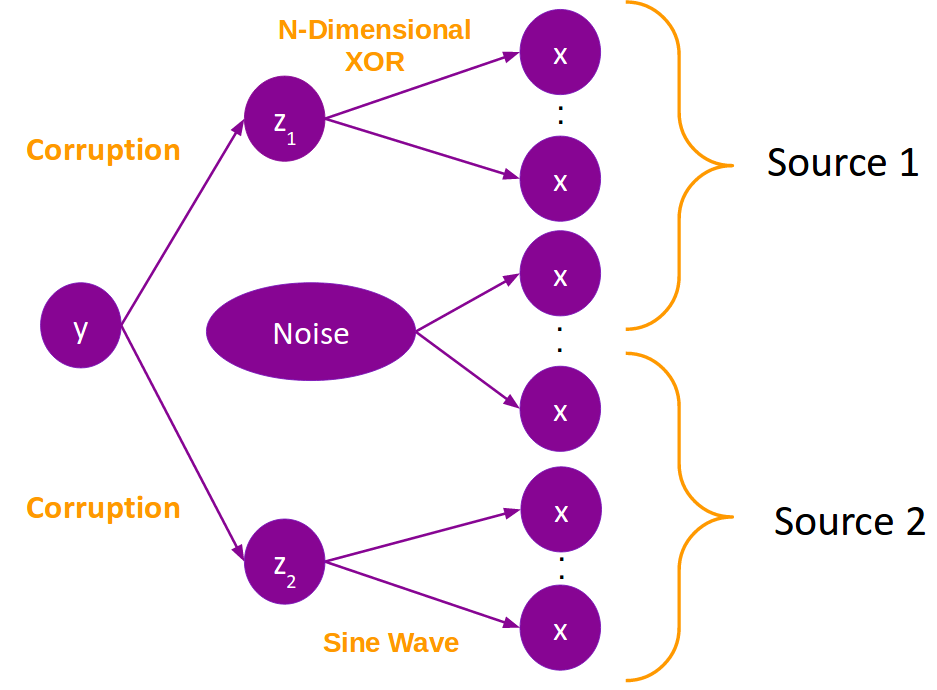
\includegraphics[scale=0.4]{network_model.png}
    \captionof{figure}{Caption for this network model}
    \label{fig:network_model}
\end{minipage}

\begin{algorithm}
\centering
\begin{algorithmic}[1]
    \caption{Network Model Data Generation Process}
    \item[] \LeftComment{Sample the $y$ layer}
    \State $y \leftarrow$ Bernoulli($p$)

    \item[]
    \item[] \LeftComment{Sample the $z$ layer}
    \ForAll{$z_i \in \{z_1, z_2\}$}
        \State $c \leftarrow$ Bernoulli($p_i$) \Comment{$p_i$ chance to corrupt
            source $i$}
        \State $z_i \leftarrow c * (1-y) + (1-c) * y$ \Comment{If corrupting,
            $z_i$ will be 0 if $y$ is 1 and 1 if $y$ is 0}
    \EndFor

    \item[]
    \item[] \LeftComment{Sample the $x$ layer of source 1, an $N_1$-dimensional XOR}
    \If{$z_1$ is even}
        \State $x^{(1)}_1 ... x^{(1)}_{N_1} \leftarrow N_1$-dimensional binary
        vector of even parity
    \Else
        \State $x^{(1)}_1 ... x^{(1)}_{N_1} \leftarrow N_1$-dimensional binary
        vector of odd parity
    \EndIf

    \item[]
    \item[] \LeftComment{Sample the $x$ layer of source 2, a $k_2$-period sine wave}
    \State $x^{(2)}_1 \leftarrow $ Uniform($-k_2\pi$, $k_2\pi$)
    \State $x^{(2)}_2 \leftarrow $ Uniform($-k_2\pi$, $k_2\pi$)
    \State $x^{(2)}_3 \leftarrow (x^{(2)}_1+x^{(2)}_2)sin(x^{(2)}_1) + mz_2$
\end{algorithmic}
\caption{Data generation process for the network model}
\label{alg:network_model}
\end{algorithm}


The above model creates two sources of data with very different types of
decision boundaries.

The first source is a $N$-dimensional XOR, which consists of clusters of points
at every corner of an $N$-dimensional hypercube, where each corner belongs to a
different class than all of its $N-1$ closest neighboring corners. Figure
\ref{fig:xor} shows a 3D example. The complexity of the decision boundary is
proportional to the dimension.

The second source is a sine wave in 3D space (Figure \ref{fig:sine_wave}); the
complexity of this decision boundary is directly proportional to the period of
the wave and inversely proportional to the margin $m$ between the two classes.

\begin{minipage}{\textwidth}
\begin{minipage}{.48\textwidth}
    \centering
    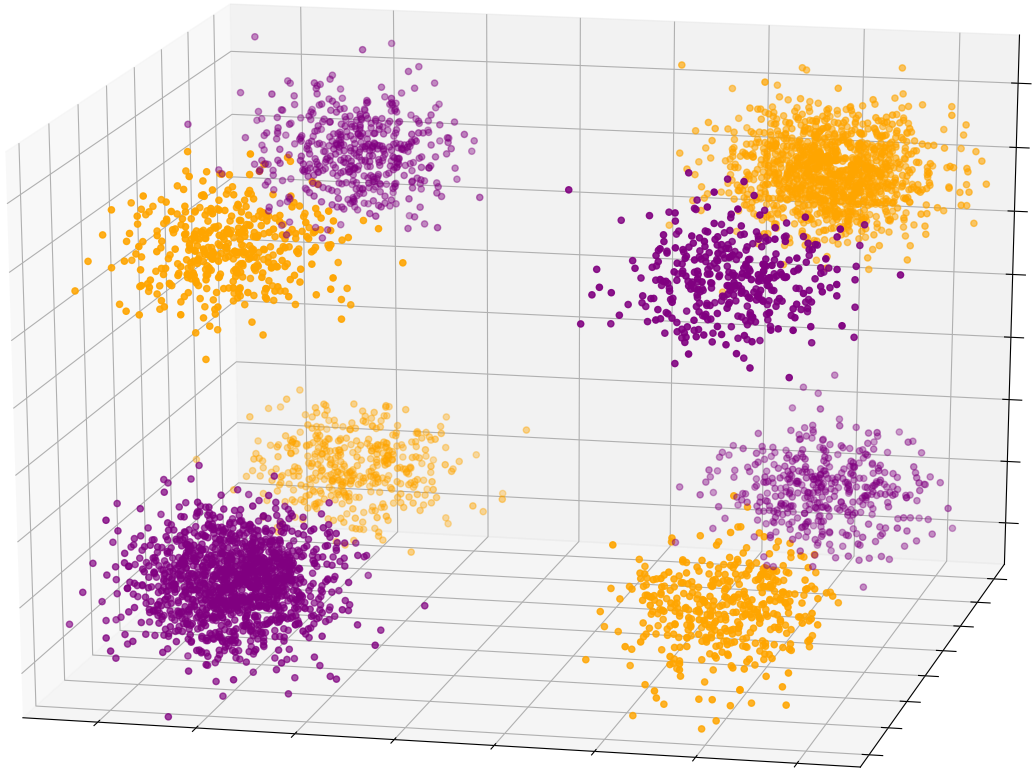
\includegraphics[width=\textwidth]{xor_3d_square.png}
    \captionof{figure}{A 3D-XOR with equal class size and $\sigma=0.2$ noise.
        The noise for the XORs created by this model are independent $Normal(0,
        \sigma)$ added to every dimension.}
    \label{fig:xor}
\end{minipage}
\hspace{.04\textwidth}
\begin{minipage}{.48\textwidth}
    \centering
    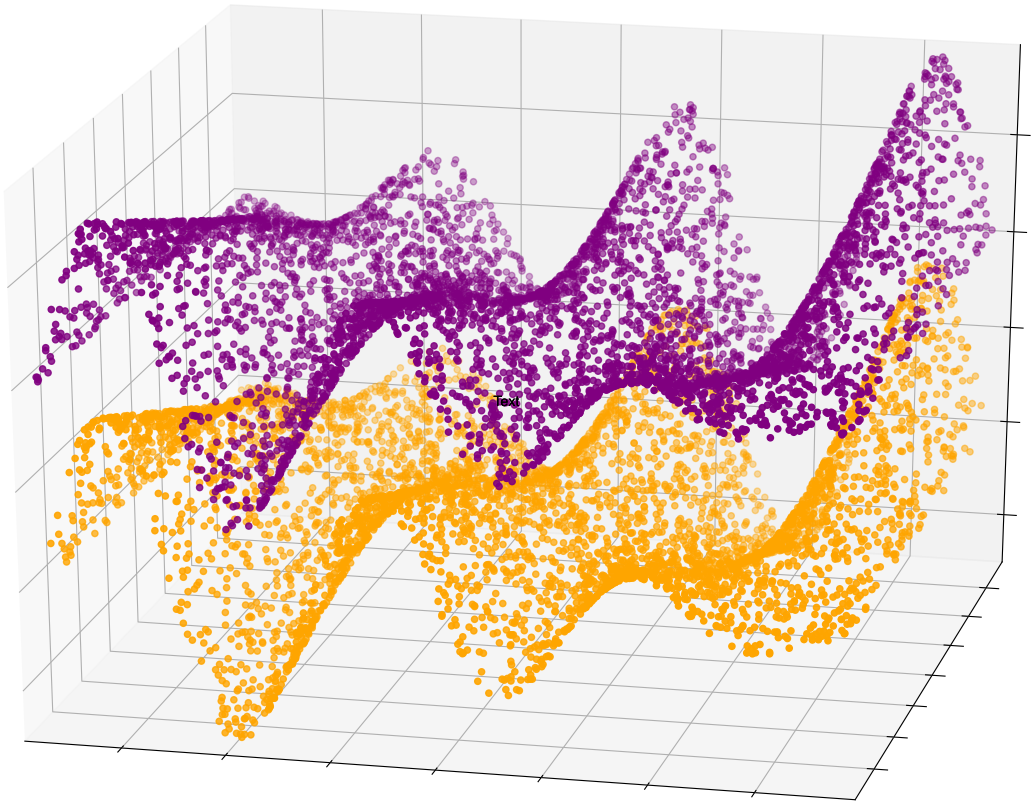
\includegraphics[width=\textwidth]{sine_wave_square.png}
    \captionof{figure}{A 3 period sine wave with $\sigma=0$ noise and a margin
        of $m=10$. The equation of this wave in xyz coordinates is $z =
        (x+y)sine(x) + mc$, where $m$ is the margin and $c$ is the 1 or 0 class
        label.}
    \label{fig:sine_wave}
\end{minipage}
\end{minipage}

In order to corrupt the sources, a Bernoulli experiment is performed for each source with a certain probability that the binomial indicator is flipped to 0 or 1 (whichever number it is currently not). A probability $p_1$ is assigned to the first source and a probability $p_2$ is assigned to the second source.  These probabilities range from 0, meaning no corruption, to 0.5, meaning complete corruption. For example, say the true value of y is 0, $p_1$ is 0, and $p_2$ is 0.5. Then the data that stems from the first source accurately represents the value of y which is 0. The data that stems from the second source will accurately represent the value of y in 50 percent of the samples, but the other 50 percent of the samples it flips to represent 1. This means that all of the information is coming from the first source while the second source tells us nothing about the true value of y.

This model has several nice properties:
\begin{itemize}
    \item For both the $N$-dimensional XOR and the sine wave (with small enough
        margin $m$), every dimension is necessary for perfect classification.
    \item The reliability of each source can be varied independently of the
        other.
    \item The data can be made more noisy (to an extent) without
        compromising the separability of the two classes.
    \item Extra meaningless dimensions can easily be added to either source.
\end{itemize}

The first experiments in this paper use a similar model to the one above, except with another XOR as the second source instead of the sinewave. The last experiments use the exact model above.











\section*{Machine Learning Classifiers}

To access the potential gain from intelligent data integration, we decided to compare the classification accuracy of a kernel based integration technique with commonly used vector concatenation benchmark algorithms.

\subsection*{Notation}
In describing different classification techniques, the following convention will be used:
\begin{itemize}
\setlength\itemsep{0em}
\item (x, y) pair denotes a feature vector x \mmin \rsup{m} and its corresponding target value $\in \{0, 1\}$ .
\item \xud{j} denotes the jth feature in x.
\item there are N training examples and $i$th training pair is represented by (\xsu{i}, \ysu{i} ).
\end{itemize}


\subsection*{Vector Concatenation Benchmarks}

\subsubsection*{Gaussian Naive Bayes}
\textbf{Model:}
The model assumes that conditioned on the value of y, every feature \xud{j} is generated independently i.e. $P(x|y) = \prod_{j=1}^{m} P(x_j|y)$. In addition it also assumes that each $P(x_j|y) \sim \mathbf{N(\mu_{j,y}, \sigma_y)}$ . To make x, the model would compute its posterior probability $P(y|x)$ and pick the more likely case.

\textbf{Properties:}
The formulation is clean and simple. It is fast to train and is quite resistant to extra noise dimensions.
However, the excessively strong assumption of independence means that we could only fit 2nd degree decision boundaries, so it is expected to perform poorly on our highly complex Double XOR dataset.

\textbf{Implementation:}
We used sklearn's Gaussian Naive Bayes classifier. No hyper-parameter tuning is required.

\subsubsection*{Random Forest}
\textbf{Model:}
The model uses an ensemble of decision trees to make a prediction for an x. Each decision tree is based by a bootstrap sample of the training data and the splitting nodes are constrained to a random subset of all features. In this manner, the over-fit of decision tree could be controlled.

\textbf{Properties:}
Random Forest is known to be very resistant to extra noise dimensions since uninformative feature would never be used for a split in a decision tree.

\textbf{Implementation:}
We used cross validation to select the optimal number of trees $\bar{t} \in \{10, 100\}$.

\subsubsection*{K-Nearest Neighbors}
\textbf{Model:}
KNN makes a prediction on an unknown data-point by the majority voting of the K-closest points i.e. $$f(x) = sign(\sum_{x^i \in \text{K closest points}} y^i) $$

\textbf{Properties:}
KNN is able to fit extremely complex decision boundaries. However, it often suffers from the curse of high dimensionality i.e. when the training data only occupies a tiny fraction of the high dimensional feature space. Moreover, it could not discriminate against noise dimensions since they are incorporated as part of the Euclidean distance.

\textbf{Implementation:}
We used cross validation to select the best number of neighbors $\bar{k} \in \{1, 10\}$




\subsubsection*{RBF Support Vector Machine}
\textbf{Model:}
Similar to KNN, Support Vector Machine makes recommendation by considering the weighted voting of a set of similar data points
$$f(x) = sign(\sum_{i=1}^{N} y^i d^i K(x, x^i))\ \text{where K(x, $x^i$)} = exp(-\gamma|x - x^i|^2)$$
where $d^i$ is learned from data by finding the largest margin separating hyperplane in the projected space.

\textbf{Properties:}
SVM can fit complex decision boundaries. Moreover, it does not suffer for the curse high dimensionality as much as KNN. Those two reasons has makes SVM the go-to algorithm for classification. However, just like KNN, it is unable to discriminate against extra noise dimensions.

\textbf{Implementation:}
Cross-validation is performed to search for the best regularization parameter $\bar{C} \in \{0.1, 1, 10, 100\}$ and $\bar{\gamma} \in \{.01, .1, 1, 10\}$




\subsection*{Generalized Multiple Kernel Learning (GMKL)}
GMKL learns separate kernels for each data source before integrating the
separate kernels in an optimization step that's based on a global error
measure; the resulting combined kernel is then fed into an SVM. Although this
method uses a SVM for actual classification, the separate kernels allow each
source to have its own representation. A brief description of the algorithm is
described below, with a general flowchart of the process shown in Figure
\ref{fig:implementation_flowchart} and a more detailed explanation of the
optimization part in Algorithm \ref{alg:gmkl}. A full explanation of the GMKL
algorithm can be found in \cite{gmkl}.

\textbf{Model:}
The final trained model is almost the same as those from SVM, expect that the final kernel function is actually learned from data. More specifically, the final kernel is a convex combination of a set of predefined kernel functions: $$K(x, x^i) = \sum_{q=1}^{Q} \theta_q * K_q(x, x^i) \text{where }\theta_q \text{is learned from data}.$$

\textbf{Formulation as Optimization Problem}
\begin{align*}
&\text{\minover{\theta, v, b}} & &C  \frac{1}{N} \sum_{i=1}^{N} L(f_{\theta, w, b}(x^i), y^i) + 1/2 \sum_{q=1}^{Q}|\frac{v_q|^2}{\theta_q} \\
&\text{subject to} & &\beta|\theta|_2^2 + (1-\beta){|\theta|_1} \leq 1
\end{align*}


Where C is the regularization parameter, $\beta$ is the elastic net parameter, L is the hinge loss function and $$f_{\theta, w, b}(x^i) = \sum_{q=1}^{Q} w_q \phi_q(x^i) \sqrt{\theta_q} + b $$
Now if we define v by $v_q := \frac{w_q}{\sqrt{\theta_q}}$, then we have a convex optimization problem:

\begin{align*}
&\text{\minover{\theta, v, b}} & &C  \frac{1}{N} \sum_{i=1}^{N} L(f_{\theta, w, b}(x^i), y^i) + 1/2 |w|^2 \\
&\text{subject to} & &\beta|\theta|_2^2 + (1-\beta){|\theta|_1} \leq 1 \\
&\text{Where}  & &f_{\theta, v, b}(x^i) = \sum_{q=1}^{Q} v_q \phi_q(x^i)  + b
\end{align*}

Observe that the elastic net constrain ensures sparsity and grouping effect for the set of kernels chosen for the final model.

\textbf{Optimization Algorithm}

\begin{algorithm}
\centering
\begin{algorithmic}[1]
    \caption{Level method for the MKL[1]}

    \item[] \LeftComment{Initialization}
    \State $t \leftarrow 0$
    \State Let $\theta$ be uniformly initialized subject to teh elastic net constraint

    \item[]
    \While{difference between the unpper bound and lower bound is less than \eps}
        \State $\alpha^{t} = \underset{\alpha}{argmax}D(\theta^{t-1}, \alpha)$
            \Comment Solve dual problem
        \State $h^t(\theta) = \underset{1 \leq i \leq t}{max} D(\theta, \alpha^i)$
            \Comment Construct a cutting plane model
        \State Calculate a lower bound and an unpper bound for the optimal solution $\overline{D_t}, \underline{D_t}$ and an improvement set level set $L = \{\theta: h^t(\theta) \leq \text{some convex combination of }\overline{D_t}, \underline{D_t}\}$
        \State Project $\theta^{t-1}$ to L to obtain $\theta^t$
    \EndWhile
\end{algorithmic}
\caption{Data generation process for the network model}
\label{alg:network_model}
\end{algorithm}

\textbf{Implementation}
For each `independent' data source, we constructed 10 RBF kernels with the width $\gamma \in \{2^{-3}, 2^{-2}, 2^{-1} ..., 2^{6}\}$. Then we trained our model with the regularization parameter $C$ fixed to 100.

\begin{minipage}{\textwidth}
    \centering
    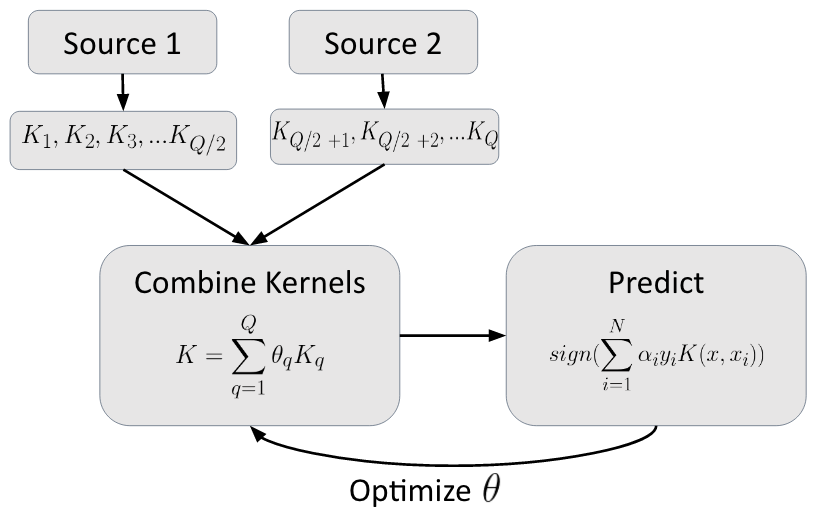
\includegraphics[scale=.4]{implementation_flowchart.png}
    \captionof{figure}{Flow Chart of Our Model}
    \label{fig:implementation_flowchart}
\end{minipage}

\textbf{Concatenated GMKL}
To isolate the effect of data integration, we also applied GMKL to concatenated data for comparison. More specifically, we constructed only 10 RBF kernels with $\gamma \in \{2^{-3}, 2^{-2}, 2^{-1} ..., 2^{6}\}$ for the concatenated dataset and then trained GMKL algorithm with C fixed at 100.\\













\section*{Experiments}



\subsection*{Experiment 1: Data Dimension Scaling}
With the prevalence of high dimensional data sets, we first would like to see
if our data integration methods scale well as the dimension of the data sources
increases. To this end, we generated several data sets of varying number of
$N_{useful}$ dimensions from a double-XOR feed-forward network. The network is
structured such that each data source receives the parity signal without
corruption from the true source, $y$. Then it creates an arbitrary n-dimensional
XOR of correct parity, which then becomes a $2n$ dimensional data vector.  A full
set of parameters for this experiment can be seen in table 4.1. This network was
chosen as it has no corruption of data sources, thus ensuring criteria 1.
Second, as the dimension of the XOR sources increase, the decision boundary becomes
increasingly complicated. Once the data generation process is complete,
classification was done by GMKL, Concatenate + GMKL, SVM, KNN, and Random
Forest.

\begin{table}
\centering
\begin{tabular}{|c c|}
\hline
Parameter & Value \\
\hline
Type of Data from each Data Source & [XOR, XOR]\\
$N_{useful}$ (For each data source) & [2,3,4,5,6,7] \\
$N_{noisy}$& 0\\
Number of Total Data points & 5000\\
Ratio of Training to Testing Data & 1:2\\
Probability of Data Source Signal Corruption & [0,0]\\
I must be missing some more parameters\\
\hline
\end{tabular}
\end{table}

\textbf{These paramters values should be replaced with the correct variable names once section 2.2.2 is completed. }\
\textbf{Should the parameters for the classifiers be described here? or in an appendix? Or in the methods section? }

\begin{minipage}{\textwidth}
\centering
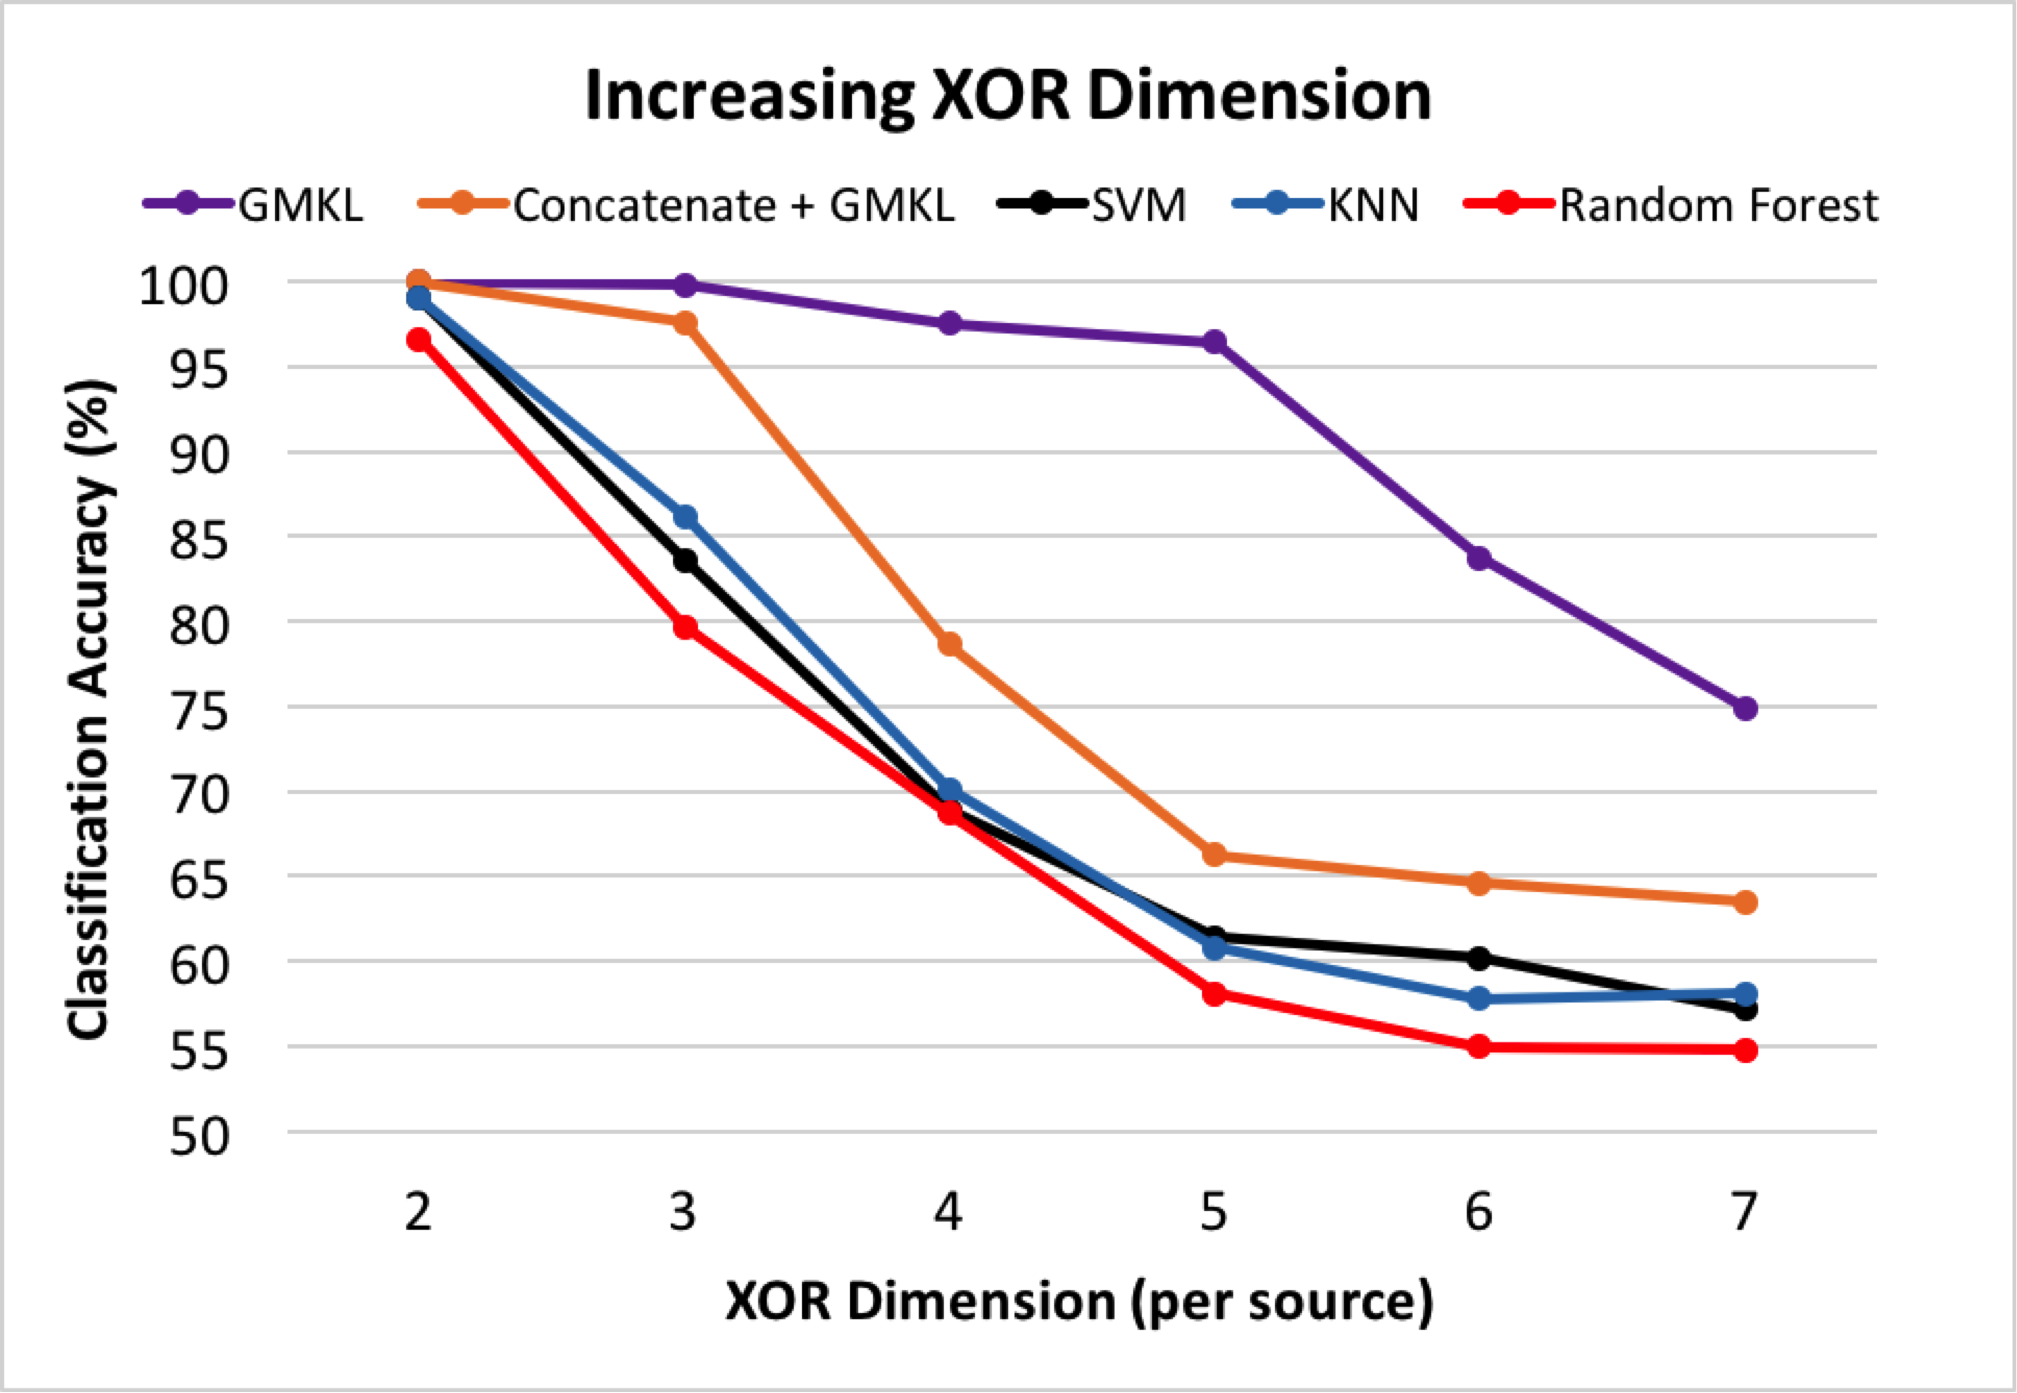
\includegraphics[scale=0.4]{experimentpic1.png}
\captionof{figure}{\textbf{PUT A CAPTION OR PARAMS OR SOMETHING HERE}}
\label{fig:exp_1}
\end{minipage}


From Figure \ref{fig:exp_1} we can see that as number of XOR dimensions increases, the classification accuracy of all of the classifiers decreases. This makes sense as the dimensionality of the data is increased without a corresponding increase in the number of data points, making the classifiers suffer from the curse of dimensionality. However, while all classifiers have decreasing accuracy, we can see that GMKL performs much better than the other classifiers with nearly a 35 percent better classification accuracy compared to the classical SVM at five dimensions. In fact, there is a very intriguing pattern on display here as the the GMKL at $2n$ dimensions seems to be performing about as well as the classical SVM at $n$ dimensions. This seems to indicate that maybe doing classification on the data sources as separate entities is highly desirabel for complicated classification problems.

\begin{minipage}{\textwidth}
\centering
\begin{tabular}{|c| c| c| c| c| }
\hline
GMKL Dimension & Accuracy & SVM Dimension & Accuracy & Difference \\
\hline
2 & a & 4 & a \\
\hline
3 & a & 6 &a
\end{tabular}
\end{minipage}










\subsection*{Experiment 2: Corrupted XOR Sources}

One variable that we decided to vary is the relative importance of the disparate sources. The purpose of this experiment is to evaluate how the various classifiers perform when one source is more important than the other. We want to see which classifers are able to identify the important sources/features.

In order to test how the classifiers perform with different level of corruption on the Double XOR data, we varied the probability of corruption for each XOR source in increments of 0.1 from 0 to 0.5. We performed this experiment three times, holding the dimension of each source static at three, five, and seven. The results of this experiment performed on five dimensional XOR are displayed in the table below. See the appendix for the results from the three dimensional and seven dimensional experiments.


\begin{minipage}{\textwidth}
    \begin{minipage}{.5\textwidth}
        \centering
        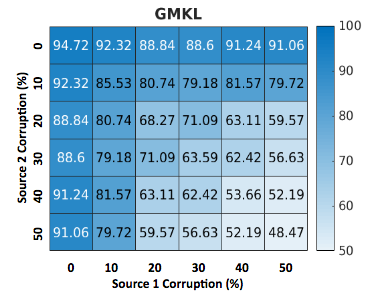
\includegraphics[width=\textwidth]{dxor_heat_gmkl.png}
        \captionof{figure}{Put a caption here}
        \label{fig:dxor_heat_gmkl}
    \end{minipage}
    \begin{minipage}{.5\textwidth}
        \centering
        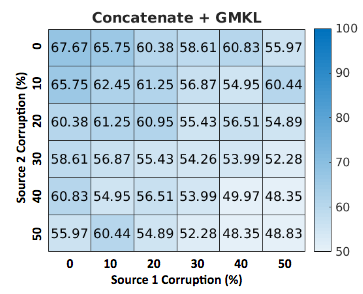
\includegraphics[width=\textwidth]{dxor_heat_conc.png}
        \captionof{figure}{Put a caption here}
        \label{fig:dxor_heat_conc}
    \end{minipage}
\end{minipage}

We see that the results of Experiment 2 are consistent with the results of Experiment 1 in that GMKL consistently outperforms concatenated GMKL which consistently outperforms the standard classifiers. We also see that GMKL is the least affected by one of the two sources becoming corrupted. This is evidence that GMKL effectively identifies which sources are useful and relies primarily on those sources.



\subsection*{Experiment 3: Noise Dimensions}

Another variable to explore is the number of noisy dimensions. This experiment explores how each classifier is able to handle additional dimensions that do not provide useful information regarding the class each point belongs to. Ideally, the classifiers are able to identify them as noise dimensions and ignores these dimension in their predictive model.

For this experiment, we added the same number of noise dimensions to each XOR source. We performed this experiment three times, when there were three, five, and seven XOR dimensions. We varied the proportion of dimensions that were noise dimensions. The proportion varied from no noise dimensions, to a quarter, third, half, and then finally two thirds noise dimensions. The purpose of measuring the proportion of noise variables as opposed to the number of noise variables is so that the three experiments over different XOR dimensions can be accurately compared.

The results from the three dimensional Double XOR experiment are represented in Figure \ref{fig:noise_dim_line}. The results from the five dimenional and seven dimensional XOR can be found in the appendix.

\begin{minipage}{\textwidth}
    \centering
    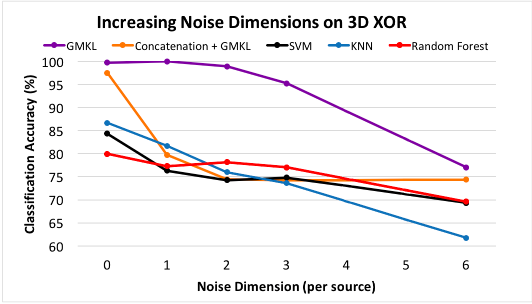
\includegraphics[scale=0.7]{Noise_Dim_line.png}
    \captionof{figure}{Put a caption here}
    \label{fig:noise_dim_line}
\end{minipage}

The purple line in the plot above shows how noise resistant GMKL is while the accuracy of Concatenated GMKL falls when only a single noise dimension is added. When there are the same number of noise dimensions as there are useful dimensions, the accuracy of GMKL is still greater than 95 percent. This tells us that GMKL effectively ignores noise dimensions. It is worthy to note the Random Forest classifier is considered noise resistant and is even less affected by noise than GMKL. However, GMKL is initially so much more accurate than Random Forest, that as far as we tested, the accuracy of GMKL remains superior to the Random Forest classifier.



\subsection*{Experiment 4: Corrupted Sine and XOR Sources}

This experiment follows the same structure as Experiment 2 in terms of varying the corruption probabilities to each source. The difference in that instead of using two sources with the XOR structure, one XOR source was used and one Sine sources was used. We also varied the corruption probabilities in different increments. The corruption probability on each source ranged from 0 to 0.45 in increments of 0.15. We executed this experiment on three dimensional XOR and Sine data with a period of two. The results are displayed below.

\begin{minipage}{\textwidth}
    \centering
    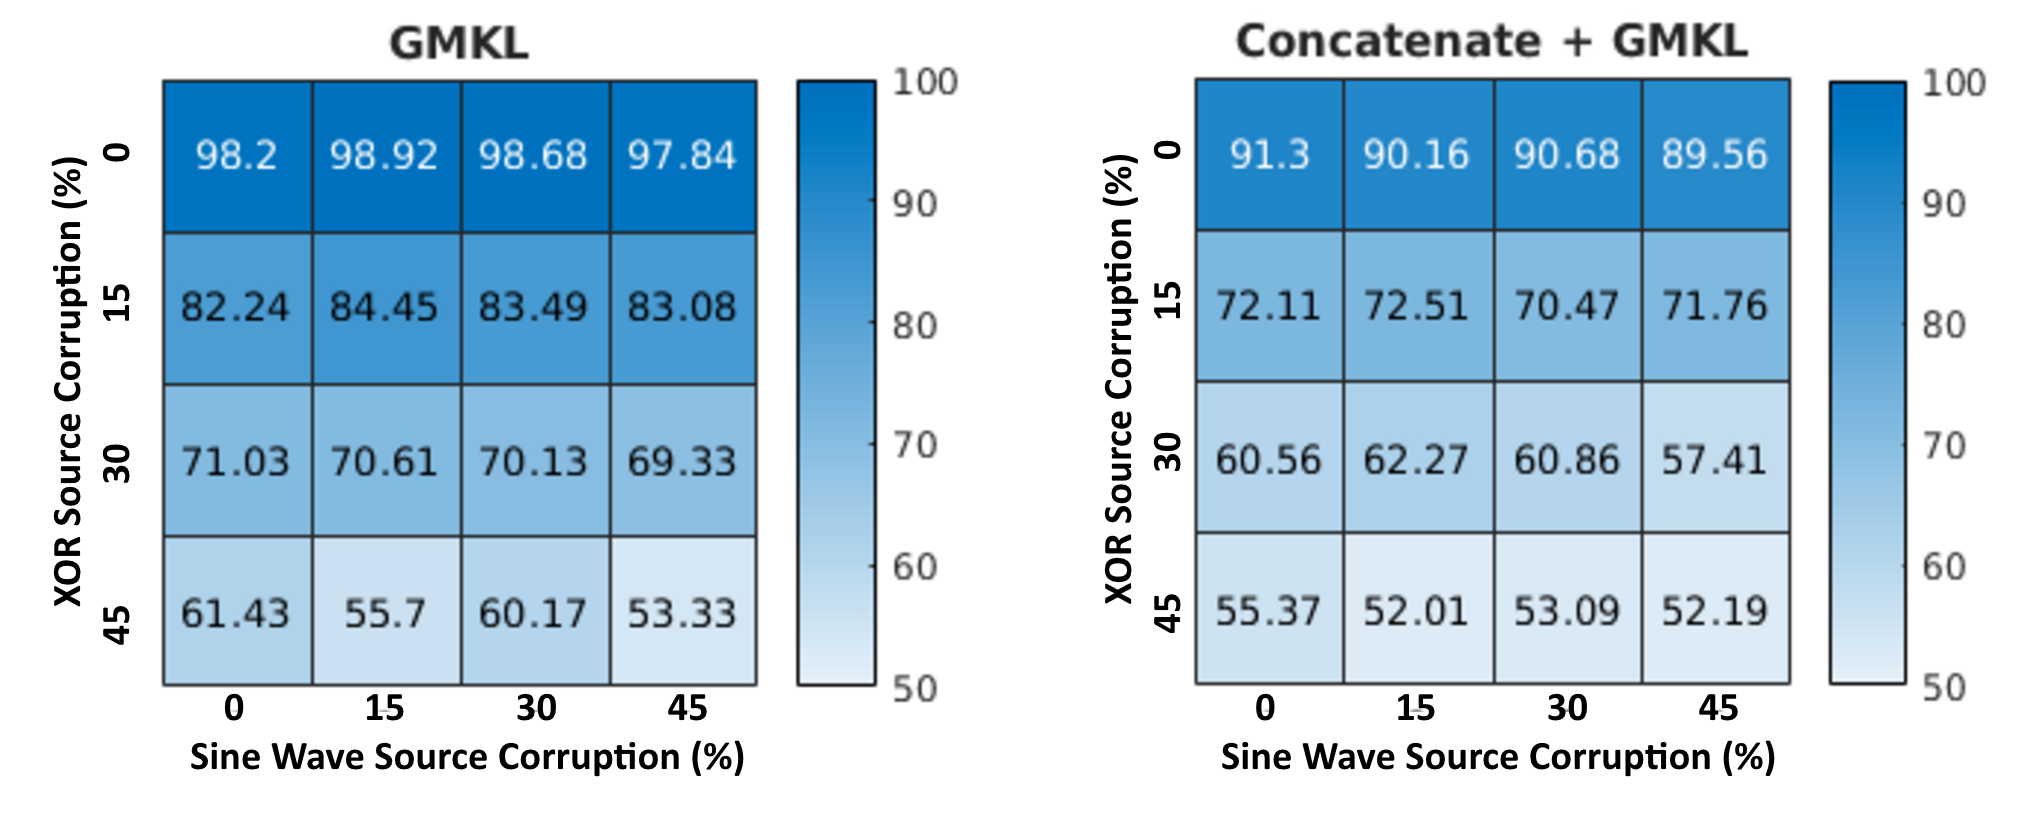
\includegraphics[width=\textwidth]{SineXORCorrupt.png}
    \captionof{figure}{Put a caption here}
    \label{fig:sinexor_heatmaps}
\end{minipage}


Again we can see that GMKL outperforms Concatenated GMKL overall. From the heat maps above, we can observe that GMKL does not handle Sine data well. When the XOR source is heavily corrupted, the prediction accuracy of GMKL falls to barely better than a coin flip. On the opposite end of the heat map, we can note that GMKL performs very well when the Sine source is heavily corrupted as long as the XOR source remains intact. This means that GMKL is insensistive to unreliable data. GMKL is successfully able to identify the source that does not contribute to classification accuracy and ignore it.

\section*{Conclusion}
From these experiments we have seen not only the usefulness of GMKL, but also the issues that traditional classifiers face in data integration. Higher dimensional data, corrupted data sources, noisy dimensions, and variably useful data sources have all been shown to negatively effect the classification accuracy of traditional classifiers such as KNN, SVM and random forest. Not only does this illustrate the usefulness of GMKL as a tool for classification and data integration, but the way in which GMKL generates kernels separately indicates the importance of treating your data sources as separate entities and the damage you will do to your classification accuracy if you concatenate it all together without any thought.


\section*{Future Work}
Data integration, data simulation, and benchmarking of machine learning techniques are all fields in need of further investigation. In particular, the behavior of machine learning and data integration techniques as functions of properties of the data and its decision boundaries is very poorly understood. Some fruitful further questions for research include:

\begin{itemize}
    \item \textbf{Shared Information Across Sources:} An important component of
        real world multi-source datasets is that information is shared across
        sources. That is, the sources aren't completely independent of each
        other, but both give insights into similar underlying hidden variables.
        The current data generation network model presented above does not have
        a way to systematically vary the information that is shared between
        both sources, but it would be very interesting to investigate if
        and how this property of the data affected the performance of
        classifiers.
    \item \textbf{Neural Networks:} Artifical neural networks are very powerful
        classifiers that are growing in popularity. They are an extremely
        extensible and flexible framework, with specialized versions existing
        for specific problems within the machine learning. They were not
        included in these experiments because they are too flexible. Neural
        networks have many more parameters than most popular classifiers, so it
        was not known how to pick an appropriate network architecture and
        topology for comparison against the other classifiers.
    \item \textbf{Theoretical Framework of Decision Boundaries:} We saw in
        Experiement 4 that GMKL performed well on the XOR dataset and not well
        on the Sine dataset. We would like to develop a theoretical framework
        that characterizes the aspects of decision boundaries that enable or
        disable a particular data integration technique from performing well on
        a dataset. We would like to come up with a concrete method for
        determining the best choice of data integration technique for a
        specific decision boundary.
    \item \textbf{More Computationally Expensive Testing:} All of the
        experiments in this paper ran with $N=5000$ data points. For really
        thorough results, it'd be better to run these experiments for several
        values of $N \in \{1000, 5000, 1000, 2000, 50000, 10000\}$ as well as
        for more values of noise, more dimensions, more corruption levels, more
        width $\gamma$ and regularization $C$ of the SVMs, etc.
    \item \textbf{More varied simulated data:} This paper only used two types
        of decision boundaries, that of the sine wave and that of the
        $N$-dimensional XOR. There are many types of decision boundaries that
        are not represented here and many possible properties of data that
        aren't present here. Possible unimplemented ideas were to create
        separable data in $m < N$ dimensions and then to use (mostly) monotonic
        transformations to map the $m$ dimensions into $N$-dimensional space,
        to create $N$ dimensional separable data.
\end{itemize}






\newpage
\section*{Appendix}

\begin{center}
\begin{tabular}{|c|c|}
\hline
\textbf{Variable} &\textbf{ Description}\\
\hline
\hline
$M_{i,useful}$ & Number of useful Data Dimensions for Data Source i\\
\hline
$M_{i, noisy}$ & Number of Noisy Dimensions for Data Source i\\
\hline
$N$ & Number of Data points Generated (training and testing)\\
\hline
T & Ratio of Training to Testing \\
\hline
$p_1, p_2$ & Probability of Data Source Corruption\\
\hline
$\sigma_i$ & Variance of Gaussian Noise \\
\hline
C & Proportion of Data points in each class \\
\hline
k & Period of Sine Curve\\
\hline
\end{tabular}
\end{center}

\subsection*{Experiment 1 Parameters}
\begin{center}
\begin{tabular}{|c|c|c|c|c|c|c|c|}
\hline
$M_{i,useful}$ & $M_{i, noisy}$ & $N$ & T &  $p_1, p_2$ & $\sigma_i$ & C &  k  \\
\hline
0& 0 & 0 &0 & 0,0 & 0 & 0 & 0  \\
\hline
\end{tabular}
\end{center}

\subsection*{Experiment 2 Parameters}
\begin{center}
\begin{tabular}{|c|c|c|c|c|c|c|c|}
\hline
$M_{i,useful}$ & $M_{i, noisy}$ & $N$ & T &  $p_1, p_2$ & $\sigma_i$ & C &  k  \\
\hline
0& 0 & 0 &0 & 0,0 & 0 & 0 & 0  \\
\hline
\end{tabular}
\end{center}
\subsection*{Experiment 3 Parameters}
\begin{center}
\begin{tabular}{|c|c|c|c|c|c|c|c|}
\hline
$M_{i,useful}$ & $M_{i, noisy}$ & $N$ & T &  $p_1, p_2$ & $\sigma_i$ & C &  k  \\
\hline
0& 0 & 0 &0 & 0,0 & 0 & 0 & 0  \\
\hline
\end{tabular}
\end{center}
\subsection*{Experiment 4 Parameters}
\begin{center}
\begin{tabular}{|c|c|c|c|c|c|c|c|}
\hline
$M_{i,useful}$ & $M_{i, noisy}$ & $N$ & T &  $p_1, p_2$ & $\sigma_i$ & C &  k  \\
\hline
0& 0 & 0 &0 & 0,0 & 0 & 0 & 0  \\
\hline
\end{tabular}
\end{center}

% \cite{gmkl}
\bibliographystyle{alpha}
\bibliography{mlsiml}

\end{document}

